%!TEX root = ../dissertation.tex
\begin{savequote}[75mm]
Language is a process of free creation; its laws and principles are fixed, but the manner in which the principles of generation are used is free and infinitely varied.
\qauthor{Noam Chomsky}
\end{savequote}

\chapter{Dynamic Multimodal Network}

\newthought{On this chapter, a new model to handle language and vision features to define a segmentation mask is proposed}, by merging previous ideas and insights (as they were described on Chapter \ref{chap:previous_work}) with state-of-the art models in both visual and language recognition tasks. This model shall take the name of Dynamic Multimodal Network (DMN), as it not only processes language and visual information in a recurrent fashion \cite{li2017cvpr} (Multimodal Network) by taking visual and language information as a concatenated entity \cite{hu2016segmentation}, but it also generates and applies a set of dynamic filters based on the language representation to the visual one at each time step, inspired on \cite{liu2017segmentation}. Additionally, a new sampling module is proposed, based on the effectiveness of skip connections \cite{DBLP:journals/corr/RonnebergerFB15} to refine and produce segmentation masks that fit each object contour accordingly.


\begin{figure}
\centering
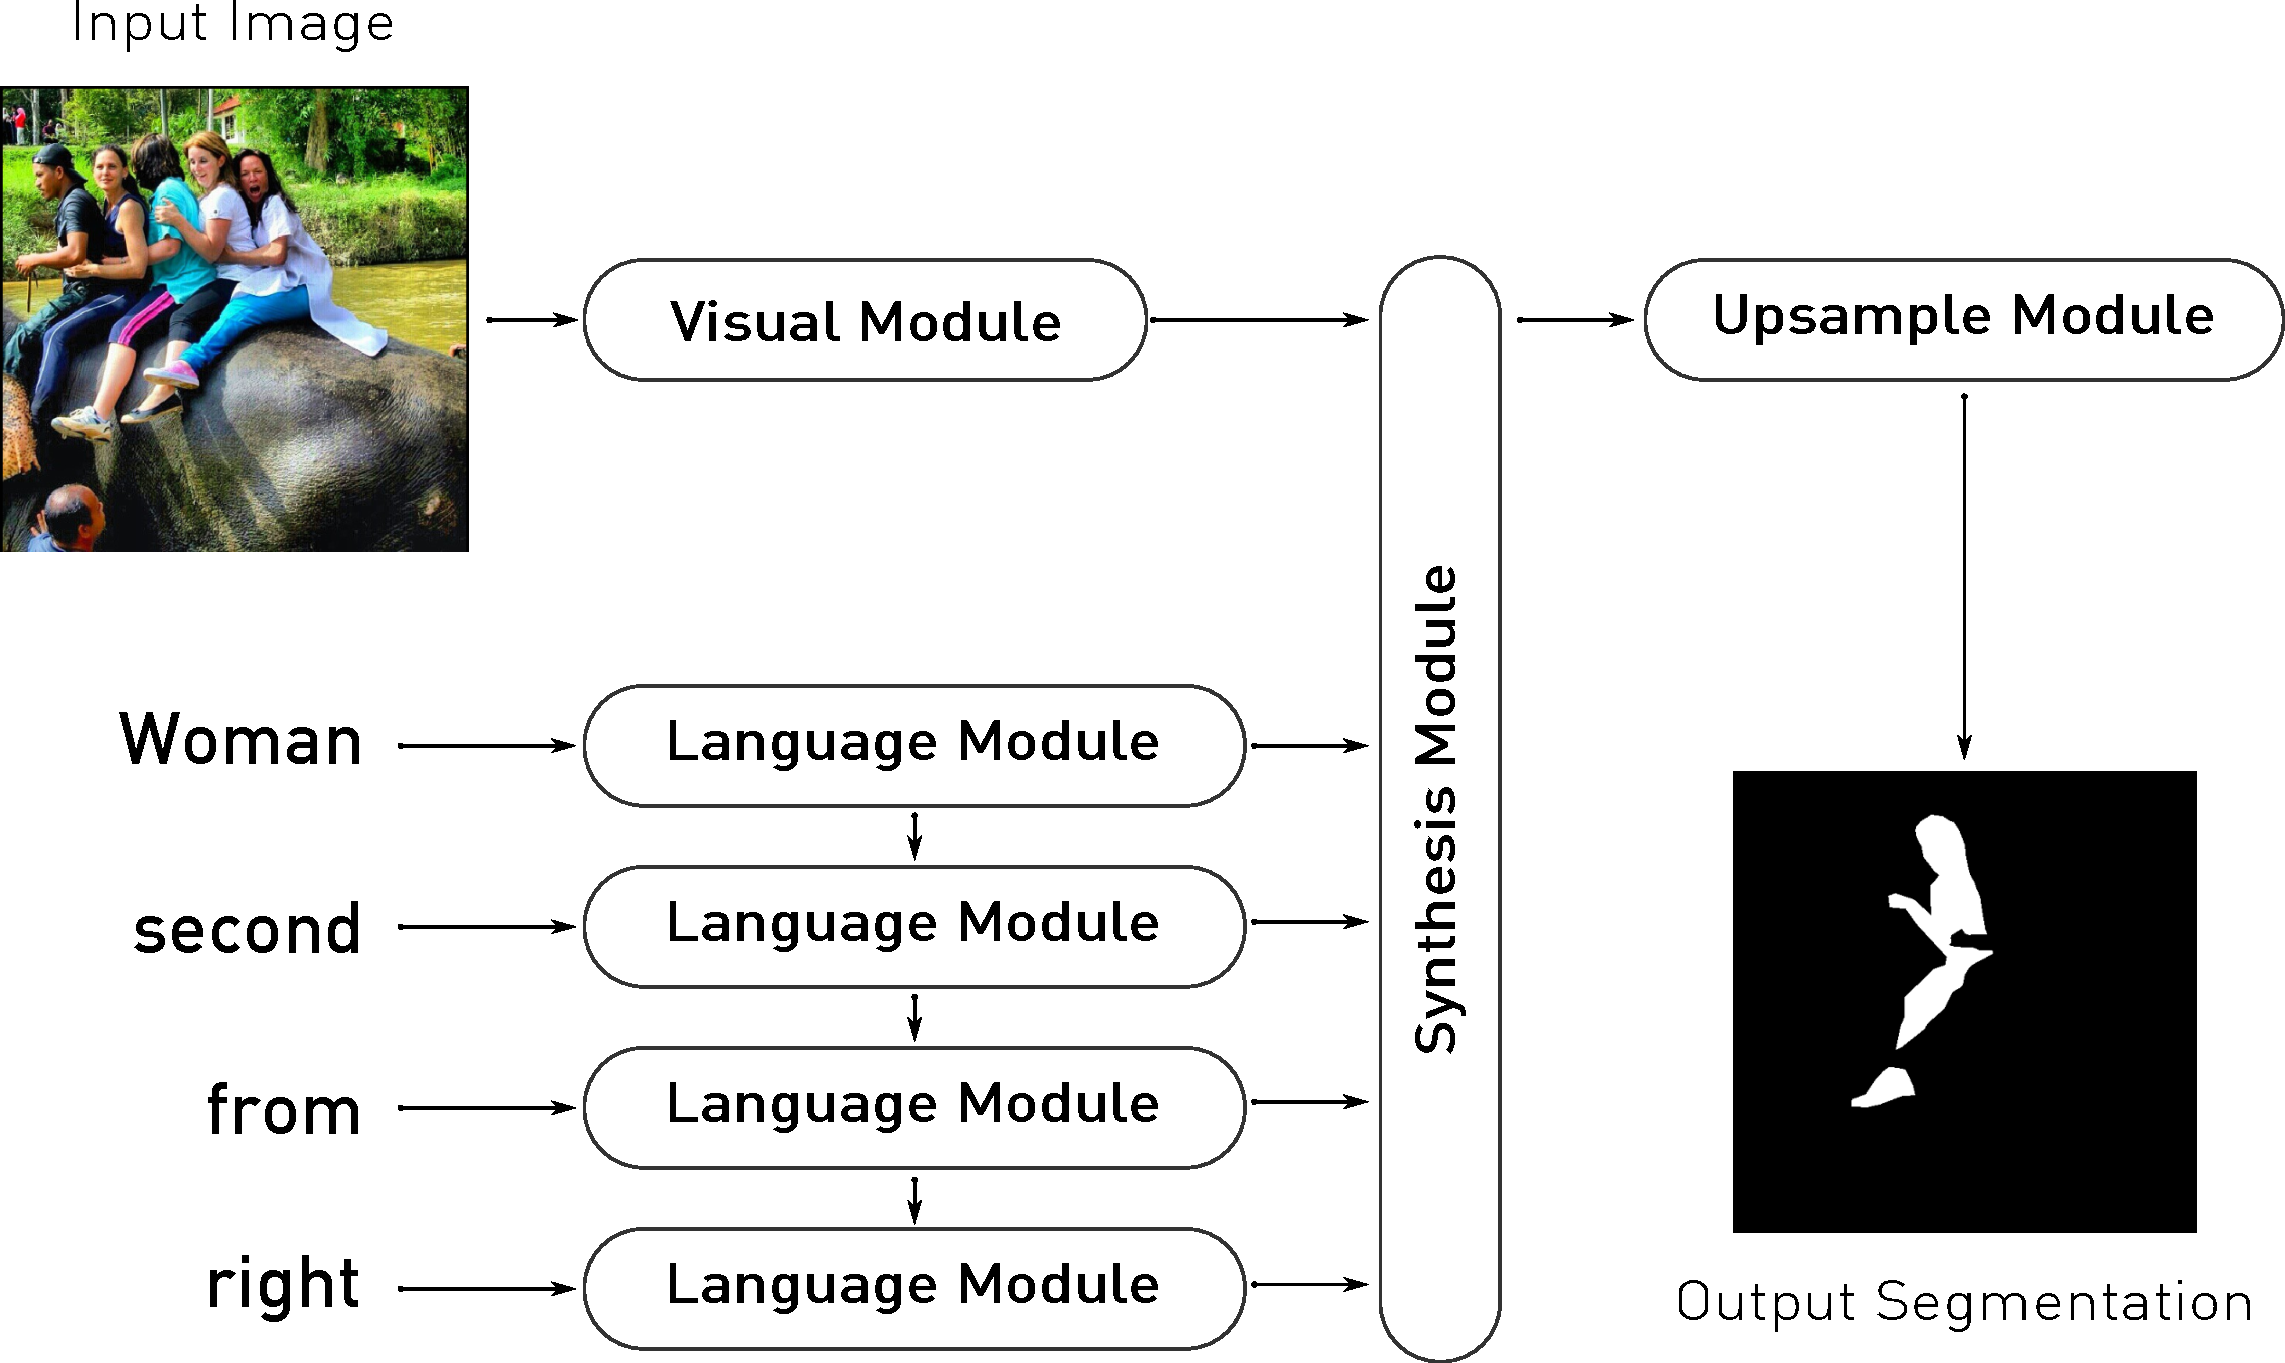
\includegraphics[width=\textwidth]{./figures/Model_Overview.pdf}
\caption{Dynamic Multimodal Network general overview consisting of a Visual Module, a Language Module, a Synthetic Module and a Upsampling Module}
\label{Fig:Overall}
\end{figure}

As shown on Figure~\ref{Fig:Overall} The DMN consists of four modules, one per each subtask proposed. The first two modules (Visual and Language modules\footnote{VM and LM, respectively}) handle each input to the model separately, extracting and modelling a representation for each modal input. Then, the Synthetic Module (SM) takes both representations and combines them to generate a low resolution segmentation mask. Finally, the Upsampling Module (UM), produces a higher resolution mask based on the output of the previous module.

The model consists of a Fully Convolutional Network (FCN) model for the VM and two Recurrent Neural Networks for the LM and the SM. The UM consists of a sequence of Convolution and Bilinear Upsampling layers that produce a $(H, W)$ mask from a low resolutuion mask of size $(\frac{H}{32}, \frac{W}{32})$. On sections \ref{section:vm} - \ref{section:um} each module is presented and described on a more detailed way.

\section{Visual Module (VM)}
\label{section:vm}

\begin{figure}
\centering
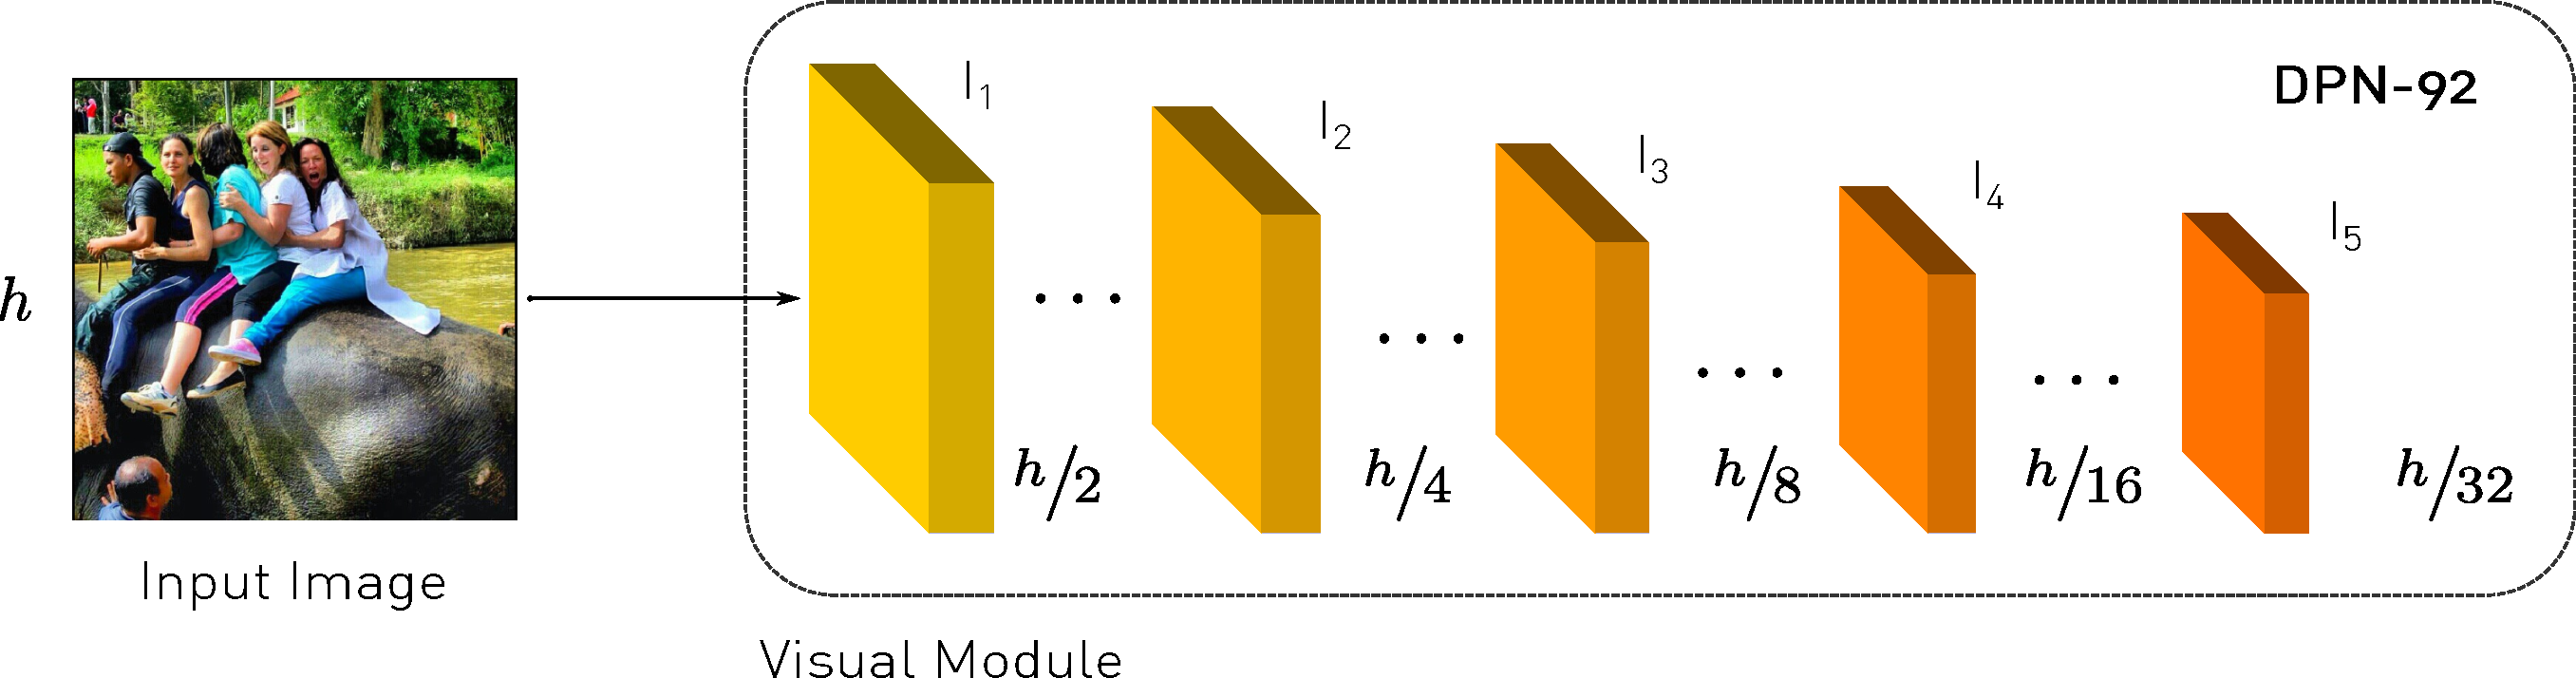
\includegraphics[width=\textwidth]{./figures/Visual_Module.pdf}
\caption{Visual Module overview}
\label{Fig:VM}
\end{figure}


The Visual Module (Figure~\ref{Fig:VM}) extracts features from an input image using a Fully Convolutional Network (FCN), these kind of models are able to take as input images of different dimensions, and therefore enables the DMN to process images of any arbitrary size. As the model depends on the multiscale features produced by the FCN, it is expected that as the FCN model improves its performance, as the visual features extracted from an input image should be more descriptive. Given this idea, the DMN experiments were based on the Dual Path Network-92 (DPN-92) \cite{DBLP:journals/corr/ChenLXJYF17}, due to its competitive results in various tasks and its parameter size efficiency.

Given an input image $I$, the VM produces a 5-tuple $\{I_1, I_2, I_3, I_4, I_5\}$, where each $I_k$ corresponds to the DPN-92 features of size $\frac{H}{2^k}$. As each map contains different resolution level features, it is expected that the encoded information will help to produce better segmentation masks, by including them on the last module.


\section{Language Module (LM)}



\section{Synthetic Module (SM)}


\section{Upsampling Module (UM)}
\label{section:um}